\chapter{Battle}
\label{ch:battle}

The Battle Discipline represents years of advanced traning in combat techniques. It enables warriors to reach an understanding of the flow of battle to such a degree that he can gain advantages over their opponents. Some times that is forcing an opponent to leave an opening or positioning themselves in such a way to avoid harm. Other times it enables unprecedented focus and calmness in the midst of battle enabling precise and calculated blows.


\section{Spot Rules}

\subsection{Learning Battle}
Characters learn Battle from other characters who know the practice. It costs two Improvement Points to get access to the Battle discipline. Each technique is learnt separately.

\subsection{Learning Techniques}
Characters learn Battle Techniques from other characters who know the appropriate techniques. Learning techniques costs one Improvement Point per Magnitude point. 
%If a character knows a technique at a lower Magnitude, they only have to pay the difference in Improvement Points to gain the technique at a higher Magnitude.

The maximum number of Battle Techniques a character can learn is INT/2.

\begin{rpg-examplebox}
Bors found a master that is willing to teach him Combat Mastery. He trains with him and spends three improvement points to succeed. 
%Bors already knows Weapon Mastery at 1 Magnitude. He wants to learn Weapon Mastery 2, so he must spend only one Improvement Point to gain the technique at that Magnitude.
\end{rpg-examplebox}

Battle Techniques can be learnt from a number of sources. The most typical is from military academies but it can also be from the lone retired veteran. 

In each case the player character must be in good standing with the teacher before they will teach them a technique. If the teacher is indifferent to the player character to start with then they will first need to undertake some kind of service, which can be the focus of an adventure.

\subsection{Using Techniques}
A character can use a technique freely as part of a combat action or reaction. Only a single Battle Technique can be used per combat round. Any Battle Technique needs to be declared before the appropriate dice is rolled.

Applying a Battle Technique is always successful but you have to spend a number of Power Points equal to the Magnitude of the technique.


\subsection{Techniques Traits}
Unless otherwise stated all Techniques have the following traits.

\begin{rpg-list}
\item All techniques, unless noted, are instant and apply only for the action or reaction that are rolled for.
\item No technique can be used in combination with special attacks like Great Attack, Disarming Attack, Aim, etc.
\item They are all Non-Variable; they can only be used at the specified Magnitude.
\end{rpg-list}

%Other traits used by techniques are detailed below. 
%\begin{description}
%	\item[Single-Attack:] Applies to a single attack.
%	\item[Combat Round:] Applies for the whole combat round (for that character)
%	\item[Non-Variable:] The technique may only be used at the stated Magnitude.
%\end{description}

\section{Techniques}
The battle techniques can improve various aspects of combat. Some are improved versions of existing manoeuvres, like Improved Disarm, while other are new, like Defensive Stance. These manoeuvres make more sense to acquire for combat experts since they will already have a high skill (which is harder to increase).

\begin{center}
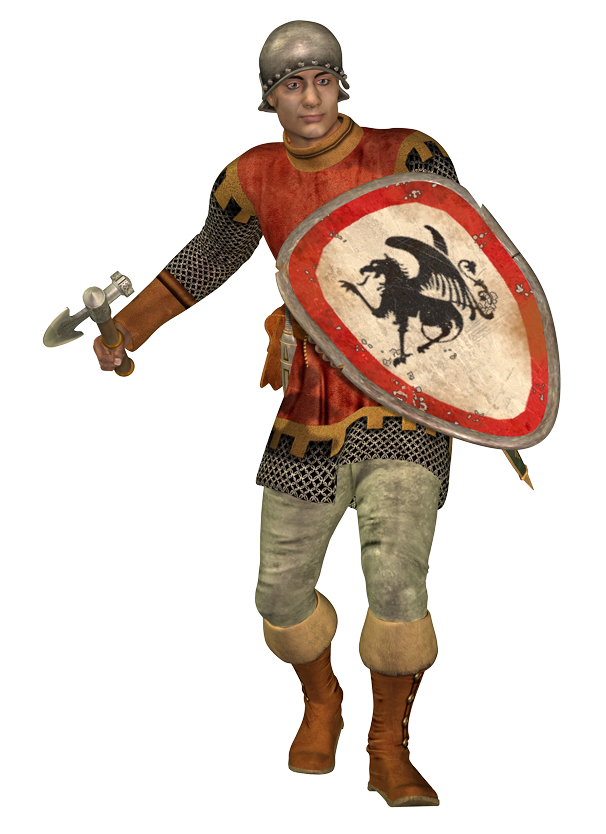
\includegraphics[scale=0.3]{img/colored/adventurer2.png}
\end{center}

\begin{table*}
\begin{center}
\caption{Battle Techniques}
\label{tab:battle-techniques}
\begin{rpg-table}[|l|c|X|]
        \hline
	\textbf{Technique} & \textbf{Magnitude} & \textbf{Effect}\\
	Awareness & 3 &  When the warrior is aware of an opponent the latter cannot gain a flanking bonus for the whole combat round.\\
	Combat Focus & 2 &  Allows a warrior to make a close combat attack with a +20\% bonus.\\
	Combat Mastery & 3 &  Allows a warrior to make a close combat attack with a +20\% bonus and +2 damage.\\
	Confuse & 2 &  Can only be used for an attack action and forces the opponent's parry or dodge to be at -20\%.\\
	Deadly Aim & 3 &  Allows a warrior to make a ranged attack with a +20\% and +2 damage.\\
	Defensive Stance & 4 &  When the warrior is wielding a shield their effective Armor Points is increased by one for the whole combat round.\\
	Impr. Combat Order & 2 &  Allows a warrior to react faster (needs to declare before combat order rolls). It provides +4 to combat order.\\% and +20\% to dodge or DEX-based Athletics tests.\\
	Impr. Aim & 2 &  The attack is similar to the Aim special attack but is immediate.\\
	Impr. All Out Attack & 4 &  The attack is similar to the All Out special attack but without losing the reaction.\\
	Impr. Disarm & 2 &  The attack is similar to the Disarm special attack but without the penalty.\\
	Impr. Great Attack & 4 &  Allows a warrior to make a Great Attack without losing their reaction.\\
	Impr. Intimidate & 2 &  The warrior's intimidate (Influence) is increased by 20\%.\\
	Impr. Knock-Back & 2 &  The attack is similar to the Knock-Back special attack but without the penalty.\\
	Impr. Knockout & 2 &  The attack is similar to the Knockout special attack but at +20\% (negating the off-hand penalty).\\
	Twin Attack & 2 &  The attack is similar to the All Out special attack but with no penalty for the first attack.\\
	Twin Missile & 4 &  Allows a warrior to make an additional single ranged attack action at -20\% in quick succession.\\
	Unarmed Fast Attack & 2 &  When unarmed a warrior can make an additional unarmed attack at -20\% in quick succession.\\
	Unarmed Focus & 2 &  Allows a warrior to make an unarmed attack with a +20\% bonus.\\
	Unarmed Mastery & 3 &  Allows a warrior to make an unarmed attack with a +20\% bonus and +2 damage.\\
        \hline
\end{rpg-table}
\end{center}
\end{table*}

